\documentclass{article}
\usepackage{graphicx} % Required for inserting images
\usepackage{float}

\title{Reproducing the Meese-Rogoff puzzle}
\author{Paul Metzler}
\date{June 2024}

\begin{document}

\maketitle

\section{Basic setup}

The Meese-Rogoff puzzle is a well-known result in the field of international finance. It refers to the fact that exchange rate models, which are based on economic fundamentals, have been found to perform poorly in out-of-sample forecasting. In this writeup, I will attempt to reproduce the Meese-Rogoff puzzle.
Spedifically, the puzzles relates to three key points:
\begin{enumerate}
    \item The nominal exchange rate follows a random walk process.
    \item The nominal exchange rate slighly negatively correlated with macroeconomic fundamentals.
    \item The nominal exchange rate is an order of magnitude more volatile than the macroeconomic fundamentals.
\end{enumerate}

I will consider the follwoing countries: United States, Euro Area, China, and United Kingdom. I will use the following macroeconomic fundamentals: Real GDP, Consumption, Inflation, and Industrial Production. The time period is from 1980 to 2019.
A details overview of the data sources is provided in the appendix.

\section{Random walk hypothesis}

To test for a random walk process, I will estimate the following model:
\begin{equation}
    \Delta s_t = \mu + \epsilon_t
\end{equation}
where $\Delta s_t$ is the change in the exchange rate, $\mu$ is the drift term, and $\varepsilon_t$ is the error term. The null hypothesis is that $\mu = 0$.
To test the null hypothesis, I will use the Augmented Dickey-Fuller test. The results are presented in Table 1.

\begin{table}[H]
    \centering
    \caption{Augmented Dickey-Fuller Test Results}
    \begin{tabular}{ccccc}
        \hline
        Currency Pair & ADF Statistic & p-value \\
        \hline
        EUR\_USD & -1.82 & 0.37 \\
        USD\_CNY & -2.32 & 0.16 \\
        GBP\_USD & -3.43 & 0.01 \\
        EUR\_CNY & -1.52 & 0.52 \\
        EUR\_GBP & -1.39 & 0.59 \\
        GBP\_CNY & -1.50 & 0.54 \\
        \hline
    \end{tabular}
\end{table}

Table 1 shows that the null hypothesis of a random walk process cannot be rejected for all currency pairs except for GBP\_USD. This result is consistent with the Meese-Rogoff puzzle.\\

Next, I will illustrate the random walk process for the EUR\_USD and the GBP\_USD exchange rate. All other currency pairs are omitted for brevity. The results are presented in Figures 1-4.

\begin{figure}[H]
    \centering
    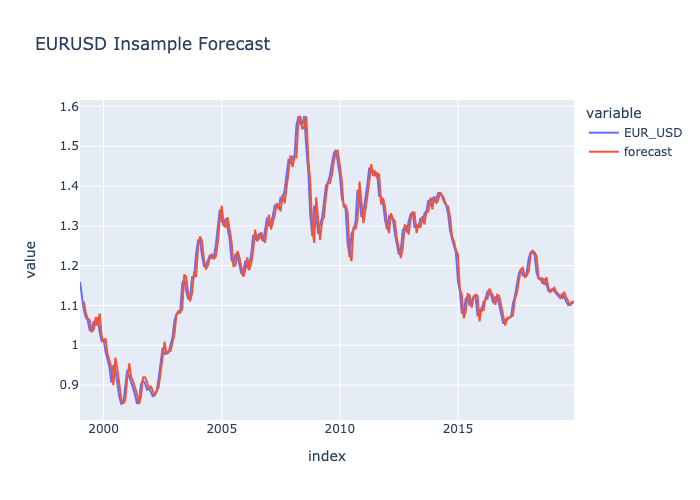
\includegraphics[width=\textwidth]{EURUSD_insample_forecast.png}
\end{figure}
\begin{figure}[H]
    \centering
    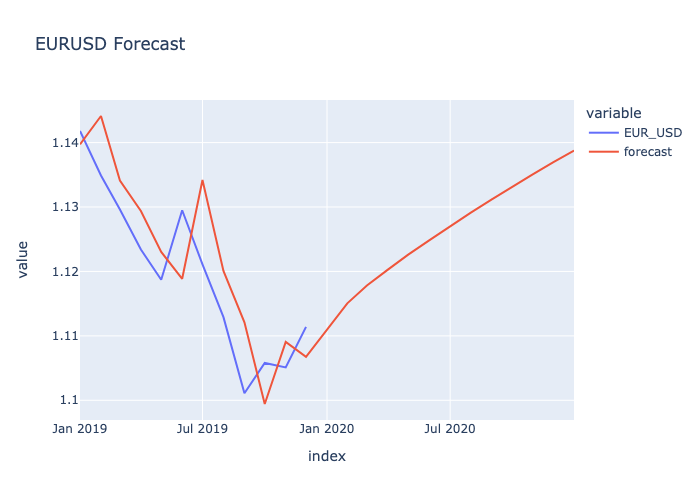
\includegraphics[width=\textwidth]{EURUSD_forecast.png}
\end{figure}
\begin{figure}[H]
    \centering
    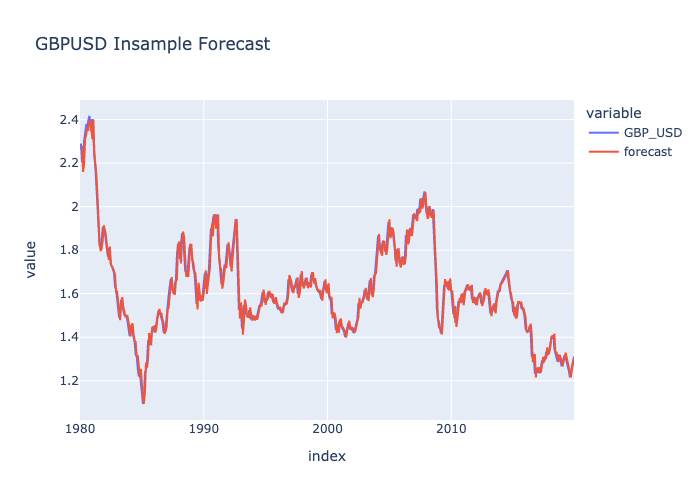
\includegraphics[width=\textwidth]{GBPUSD_insample_forecast.png}
\end{figure}
\begin{figure}[H]
    \centering
    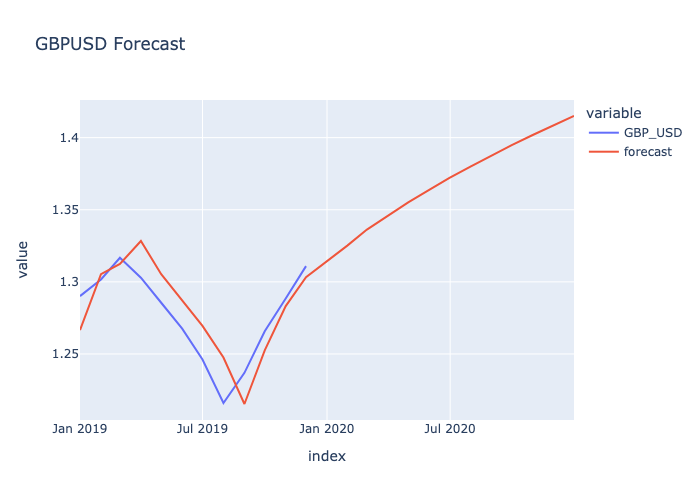
\includegraphics[width=\textwidth]{GBPUSD_forecast.png}
\end{figure}

The lag length is selected based on the Schwarz Bayesian Information Criterion (BIC) and results in a lag length of 2 for both currency pairs. 
All other currency pairs result in a lag length of 1. The coefficient estimates are presented in Table 2. The coefficient estimates are close to 1 in sum for both currency pairs, which is consistent with a random walk process.\\
\begin{table}[H]
    \centering
    \caption{Coefficient Estimates}
    \begin{tabular}{ccc}
        \hline
        Currency Pair & Coefficient & Estimate \\
        \hline
        EUR\_USD & const & 0.0223 \\
        & $EUR\_USD_{t-1}$ & 1.2863 \\
        & $EUR\_USD_{t-2}$ & -0.3048 \\
        \hline
        GBP\_USD & const & 0.0410 \\
        & $GBP\_USD_{t-1}$ & 1.3052 \\
        & $GBP\_USD_{t-2}$ & -0.3314 \\
        \hline
    \end{tabular}
\end{table}

\section{Correlation with macroeconomic fundamentals}

To test for correlation with macroeconomic fundamentals, I compute the correlation between the exchange rate and the macroeconomic fundamentals. 
The results are presented in Figures 5-8.

\begin{figure}[H]
    \centering
    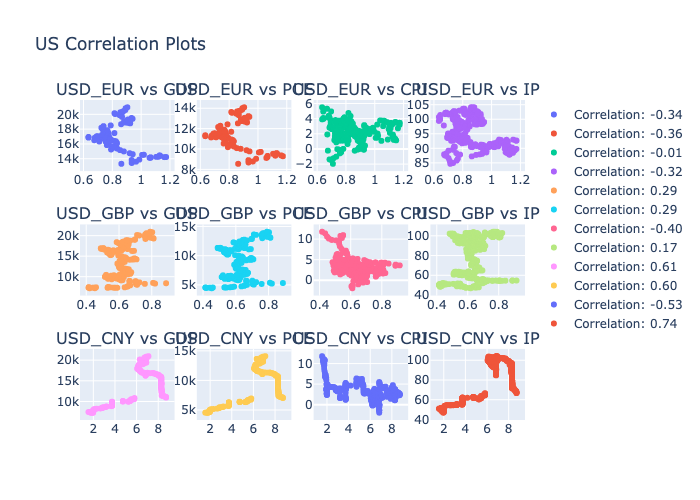
\includegraphics[width=\textwidth]{US_corr_plots.png}
\end{figure}
The US shows Meese-Rogoff behavior against Euro Area data (slightly negative correlation against real macreoeconomic aggregates). However, correlation for these variables is slighly positive against UK data and substantially positive against China's data (which could be a result of the Chinese exchange rate regime).

\begin{figure}[H]
    \centering
    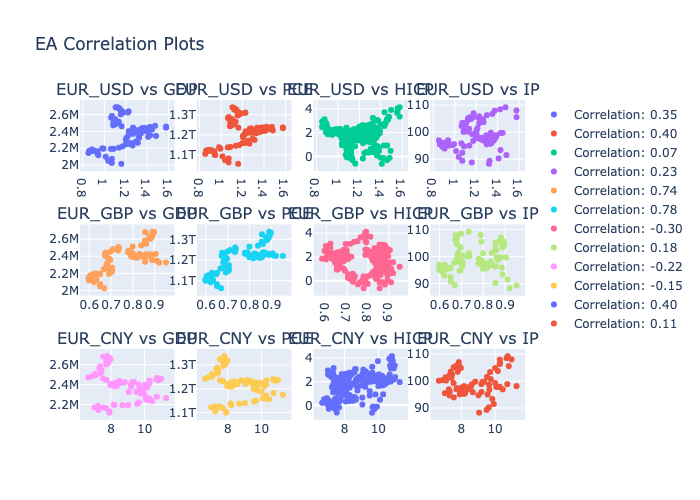
\includegraphics[width=\textwidth]{EA_corr_plots.png}
\end{figure}
The Euro area shows a slight positive correlation between the US exchange rate and real macreoeconomic aggregates. This correlation is stronger for the UK than the US. The correlation between the Chinese exchange rate and real macroeconomic aggregates is slightly negative.

\begin{figure}[H]
    \centering
    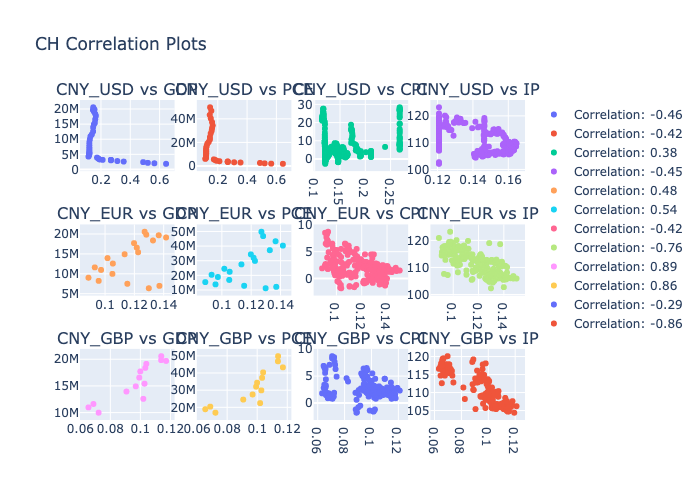
\includegraphics[width=\textwidth]{CH_corr_plots.png}
\end{figure}
China shows Meese-Rogoff behavior against the US and ambigous against UK and Euro area as GDP and consumption are substaintually (EA) and highly (UK) positively correlated but industrial production is strongly negatively correlated.

\begin{figure}[H]
    \centering
    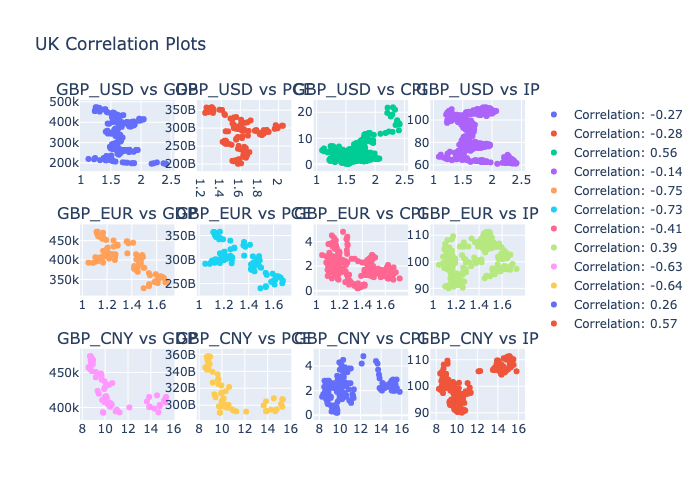
\includegraphics[width=\textwidth]{UK_corr_plots.png}
\end{figure}
The UK shows Meese-Rogoff behavior against the US. Against the Euro area and Chinese Exchange rates, when looking at GDP and consumption. The Correlation for the EA and China becomes substantially positive when looking at industrial production.\\

The mostly results are consistent with the Meese-Rogoff puzzle. The correlation between the exchange rate and the macroeconomic fundamentals is inconsistent across countries and some countries have high positive correlation as indicated by textbook predictions.\\
To test robustness, I check additional measures for Inflation in the US and the UK. The results do not change significantly. Further, I have looked at the correlation between the exchange rate and the macroeconomic fundamentals for different time periods. These results are presented below in Figures 9-20.

\subsection{2010s}
\begin{figure}[H]
    \centering
    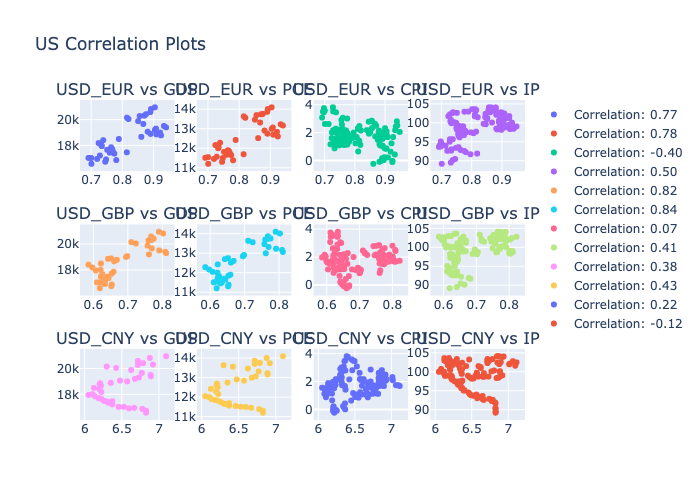
\includegraphics[width=\textwidth]{US2010s_corr_plots.png}
\end{figure}
\begin{figure}[H]
    \centering
    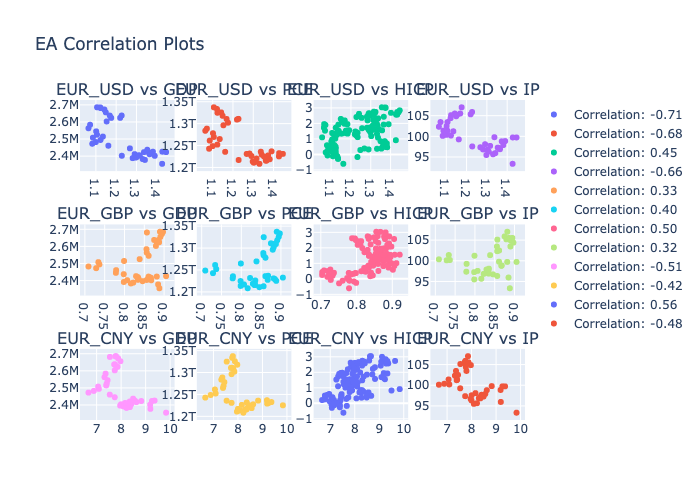
\includegraphics[width=\textwidth]{EA2010s_corr_plots.png}
\end{figure}
\begin{figure}[H]
    \centering
    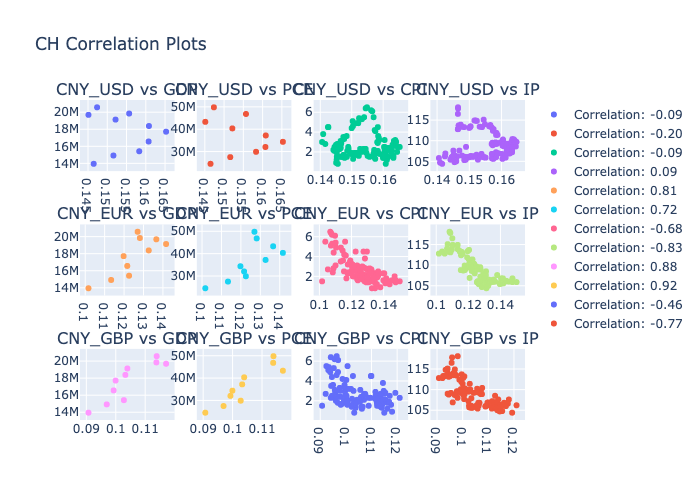
\includegraphics[width=\textwidth]{CH2010s_corr_plots.png}
\end{figure}
\begin{figure}[H]
    \centering
    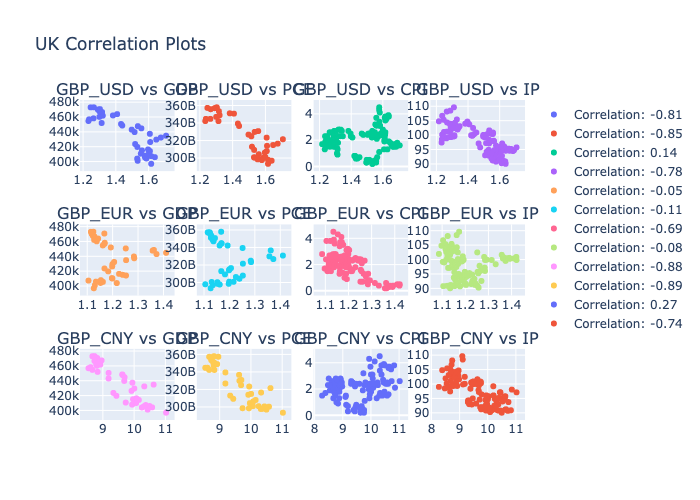
\includegraphics[width=\textwidth]{UK2010s_corr_plots.png}
\end{figure}

US has positive correlation with most macro aggregates, EA has negative against US and China but positive against UK (perhaps because of Trade in EU?). 
China has negative correlation against USD but strongly positive against other FX. UK is strongly negative against USD and CNY but only slightly negative against EUR.

\subsection{2000s}
\begin{figure}[H]
    \centering
    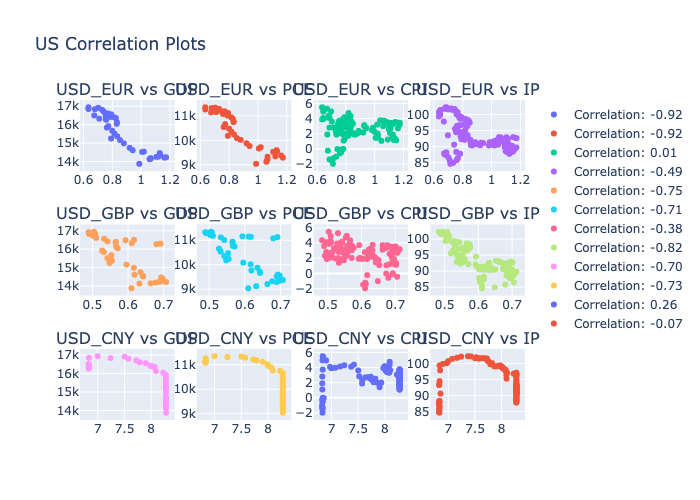
\includegraphics[width=\textwidth]{US2000s_corr_plots.png}
\end{figure}
\begin{figure}[H]
    \centering
    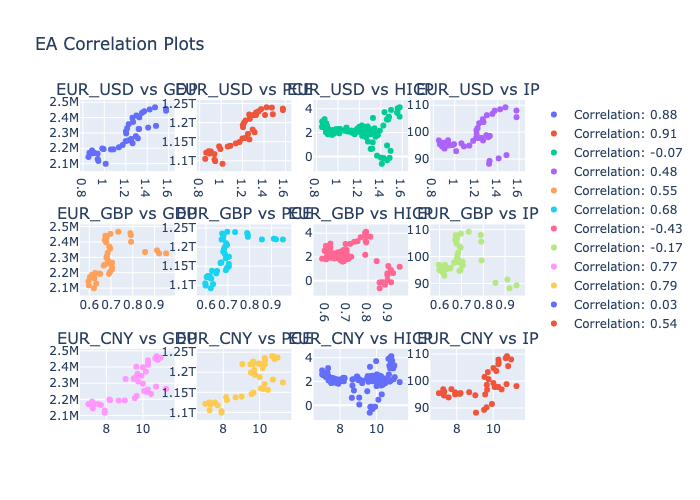
\includegraphics[width=\textwidth]{EA2000s_corr_plots.png}
\end{figure}
\begin{figure}[H]
    \centering
    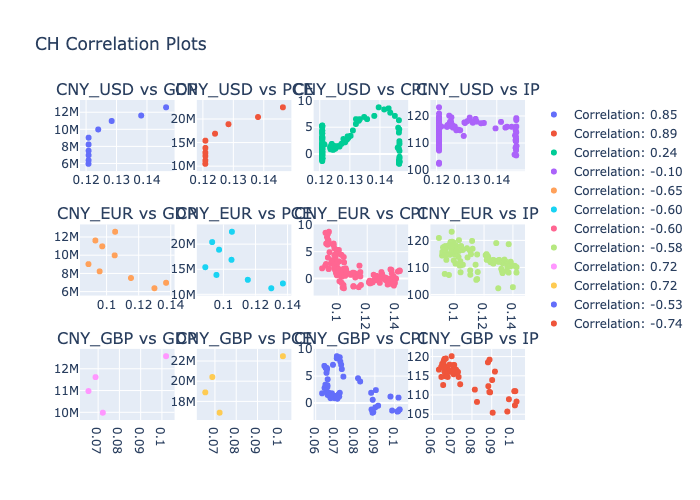
\includegraphics[width=\textwidth]{CH2000s_corr_plots.png}
\end{figure}
\begin{figure}[H]
    \centering
    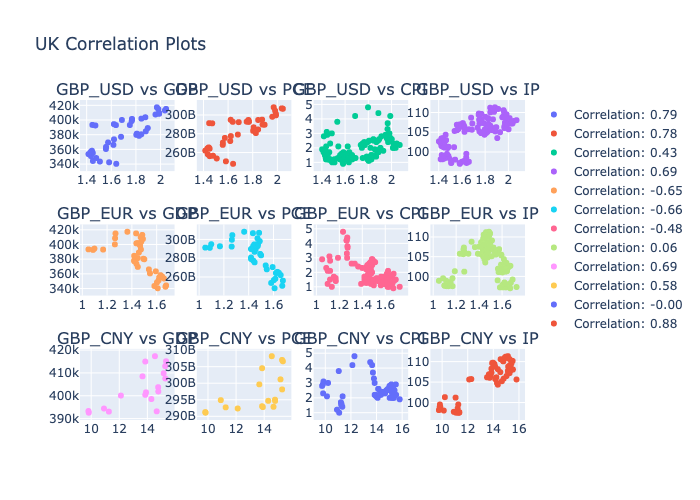
\includegraphics[width=\textwidth]{UK2000s_corr_plots.png}
\end{figure}
A mixed bag: US strongly negative to all FX rates, EA mostly positive to all FX rates, UK and China behave Meese-Rogoff style against the Euro but positively against the other FX rates.

\subsection{Pre-2000s}
\begin{figure}[H]
    \centering
    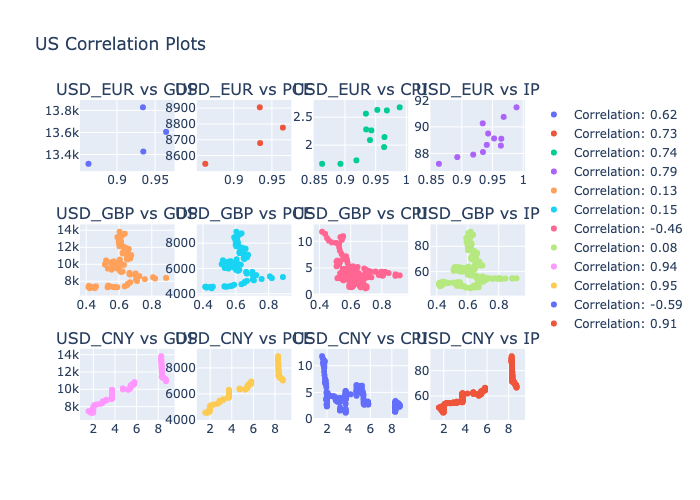
\includegraphics[width=\textwidth]{USPre2000s_corr_plots.png}
\end{figure}
\begin{figure}[H]
    \centering
    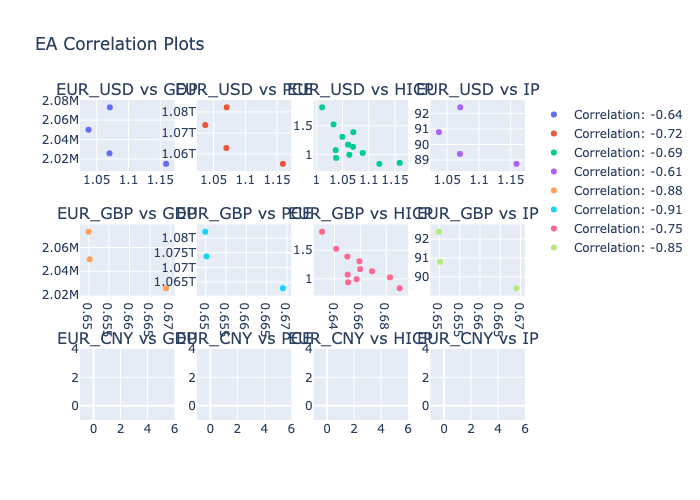
\includegraphics[width=\textwidth]{EAPre2000s_corr_plots.png}
\end{figure}
\begin{figure}[H]
    \centering
    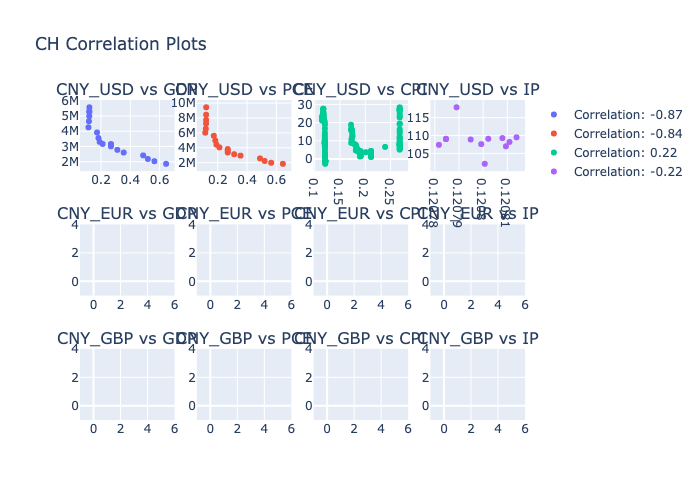
\includegraphics[width=\textwidth]{CHPre2000s_corr_plots.png}
\end{figure}
\begin{figure}[H]
    \centering
    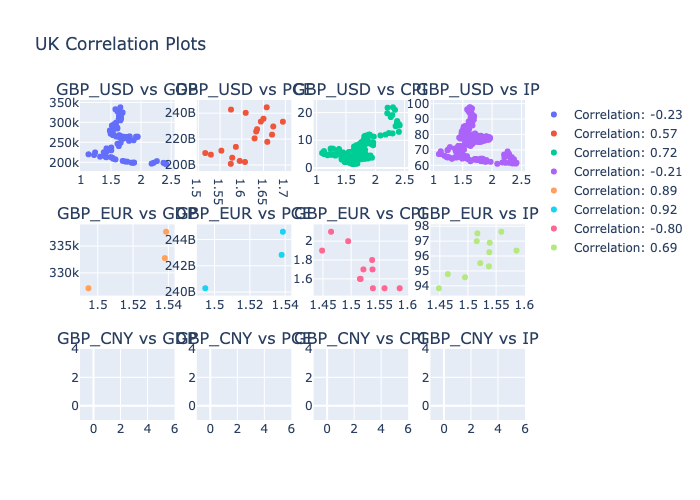
\includegraphics[width=\textwidth]{UKPre2000s_corr_plots.png}
\end{figure}

This time period has a lot of missing data, but the results are consistent with the 2000s.


\section{Volatility}
To test for volatility, I compute the coefficient of variation for the exchange rate and the macroeconomic fundamentals. The results are presented in Tables 3-4.

\begin{table}[H]
    \centering
    \caption{Coefficient of Variation for Exchange Rates}
    \begin{tabular}{cc}
        \hline
        Currency Pair & Coefficient of Variation \\
        \hline
        EUR\_USD & 0.137532 \\
        USD\_CNY & 0.340936 \\
        GBP\_USD & 0.139196 \\
        EUR\_CNY & 0.137270 \\
        EUR\_GBP & 0.131044 \\
        GBP\_CNY & 0.205771 \\
        \hline
    \end{tabular}
\end{table}
\begin{table}[H]
    \centering
    \caption{Coefficient of Variation for Macroeconomic Fundamentals}
    \begin{tabular}{cc}
        \hline
        Macro Variable & Coefficient of Variation \\
        \hline
        US\_GDP & 0.300641 \\
        US\_PCE & 0.325222 \\
        US\_CPI & 0.626225 \\
        US\_IP & 0.235516 \\
        EA\_GDP & 0.099539 \\
        EA\_PCE & 0.085062 \\
        EA\_HICP & 0.523841 \\
        EA\_IP & 0.155300 \\
        CH\_GDP & 0.733270 \\
        CH\_PCE & 0.918761 \\
        CH\_CPI & 1.324669 \\
        CH\_IP & 0.040400 \\
        UK\_GDP & 0.257143 \\
        UK\_PCE & 0.148393 \\
        UK\_CPI & 0.905414 \\
        UK\_IP & 0.164152 \\
        \hline
    \end{tabular}
\end{table}

The mean coefficient of variation for the exchange rate is \textbf{0.18}, while the mean coefficient of variation for the macroeconomic fundamentals is \textbf{0.43}. This means that (when looking at the whole time period) the exchange rate is less volatile than the macroeconomic fundamentals which is exactly opposite to the Meese-Rogoff puzzle.

\subsection{Volatility across different Time Periods}
Hence, I will look at the coefficient of variation for different time periods. The results are presented in Tables 5-6.


\begin{table}[H]
    \centering
    \caption{Coefficient of Variation for Exchange Rates for Different Time Periods}
    \begin{tabular}{ccccc}
        \hline
        {} &  1980 - 1989 &  1990 - 1999 &  2000 - 2009 &  2010 - 2019 \\
        \hline
        EUR\_USD &          n/a &     0.038167 &     0.172238 &     0.091876 \\
        USD\_CNY &     0.293248 &     0.210096 &     0.069537 &     0.043831 \\
        GBP\_USD &     0.187961 &     0.073158 &     0.116787 &     0.096420 \\
        EUR\_CNY &          n/a &          n/a &     0.132758 &     0.085562 \\
        EUR\_GBP &          n/a &     0.026397 &     0.120149 &     0.061514 \\
        GBP\_CNY &          n/a &          n/a &     0.138421 &     0.073414 \\
        Mean    &     0.240605 &     0.086954 &     0.124982 &     0.075436 \\
        \hline
    \end{tabular}
\end{table}

\begin{table}[H]
    \centering
    \caption{Coefficient of Variation for Macroeconomic Fundamentals for Different Time Periods}
    \begin{tabular}{ccccc}
        \hline
        {} &  1980 - 1989 &  1990 - 1999 &  2000 - 2009 &  2010 - 2019 \\
        \hline
        US\_GDP  &     0.110085 &     0.102729 &     0.065922 &     0.069426 \\
        US\_PCE  &     0.117490 &     0.106137 &     0.074602 &     0.071073 \\
        US\_CPI  &     0.516798 &     0.374264 &     0.552906 &     0.484439 \\
        US\_CPI2 &     0.513209 &     0.286394 &     0.181355 &     0.261563 \\
        US\_IP   &     0.084676 &     0.131911 &     0.050248 &     0.036508 \\
        EA\_GDP  &     n/a &          0.037894 &     0.047694 &     0.042144 \\
        EA\_PCE  &     n/a &          0.038603 &     0.040642 &     0.032435 \\
        EA\_HICP &     n/a &          0.248845 &     0.375226 &     0.659984 \\
        EA\_IP   &     0.060317 &     0.054538 &     0.055377 &     0.035565 \\
        CH\_GDP  &     0.207091 &     0.201474 &     0.257757 &     0.130489 \\
        CH\_PCE  &     0.279914 &     0.274381 &     0.264181 &     0.230111 \\
        CH\_CPI  &     0.562052 &     1.058059 &     1.331435 &     0.484714 \\
        CH\_IP   &     n/a &          0.032289 &     0.034552 &     0.030021 \\
        UK\_GDP  &     0.103574 &     0.082449 &     0.061948 &     0.056027 \\
        UK\_PCE  &     n/a &          0.064349 &     0.060889 &     0.067694 \\
        UK\_CPI  &     0.629939 &     0.632887 &     0.399075 &     0.465481 \\
        UK\_CPI2 &     0.549680 &     0.812161 &     0.416127 &     0.227597 \\
        UK\_IP   &     0.084472 &     0.075265 &     0.038867 &     0.049292 \\
        Mean    &      0.293792 &     0.256368 &     0.239378 &     0.190809 \\
        \hline
    \end{tabular}
\end{table}

Now, the mean coefficient of variation for the exchange rate is \textbf{0.11}, while the mean coefficient of variation for the macroeconomic fundamentals is \textbf{0.23}. This means that the exchange rate is less volatile than the macroeconomic fundamentals for all time periods.
While this is a lot closer in terms of volatility, it is still not consistent with the Meese-Rogoff puzzle.


\section{Conclusion}
In this writeup, I have attempted to reproduce the Meese-Rogoff puzzle. The results are quite mixed. The exchange rate follows a random walk process for all currency pairs except for GBP\_USD. The correlation between the exchange rate and the macroeconomic fundamentals is inconsistent across countries. The exchange rate is less volatile than the macroeconomic fundamentals for all time periods.\\

\newpage

\section*{Appendix}

This write-up provides an overview of the economic data sources for the United States (US), Euro Area (EA), China, and the United Kingdom (UK). Each section describes the specific variables used, their corresponding codes, and the sources from which the data is obtained.\\
\\
United States (US)\\
Data Sources: Federal Reserve Economic Data (FRED)\\
\\
Real GDP (GDPC1)\\
Real Personal Consumption Expenditures (PCECC96)\\
Consumer Price Index (CPIAUCSL, CORESTICKM159SFRBATL)\\
Industrial Production (INDPRO)\\
\\
Euro Area (EA)\\
Data Sources: Eurostat, OECD\\
\\
Real GDP (CLVMEURSCAB1GQEA19)\\
Real Personal Consumption Expenditures (NAEXKP02EZQ189S)\\
Harmonized Index of Consumer Prices (HICP) (CP0000EZ19M086NEST)\\
Industrial Production (PRINTO01EZQ661S)\\
\\
China\\
Data Sources: Penn World Tables, IMF, OECD\\
\\
Real GDP (RGDPNACNA666NRUG)\\
Real Personal Consumption Expenditures (NCRXDCCNA)\\
Consumer Price Index (CPI) (CPALTT01CNM659N)\\
Industrial Production (CHNPRINTO01IXPYM)\\
\\
United Kingdom (UK)\\
Data Sources: Eurostat, OECD\\
\\
Real GDP (CLVMNACSCAB1GQUK)\\
Real Personal Consumption Expenditures (GBRPFCEQDSNAQ)\\
Consumer Price Index (CPI) (CPALTT01GBM659N, CPGRLE01GBM659N)\\
Industrial Production (GBRPRINTO01GPSAM)\\
\\
Exchange Rates\\
Data Sources: FRED, European Central Bank (ECB), Bank of England\\
\\
USD to EUR (EXUSEU)\\
USD to CNY (EXCHUS)\\
USD to GBP (EXUSUK)\\
CNY to EUR (EXR.D.CNY.EUR.SP00.A)\\
GBP to EUR (EXR.D.GBP.EUR.SP00.A)\\
GBP to CNH (XUDLBK89)\\


\end{document}